\section{Introdução}

A arquitetura de sistemas digitais modernos exige componentes versáteis e eficientes para o processamento de dados. Dentre esses componentes, a Unidade Lógica e Aritmética (ALU – Arithmetic and Logic Unit) desempenha um papel central na execução de operações fundamentais como somas, subtrações, operações lógicas e manipulações de bits.

\begin{figure}[H]
    \centering
    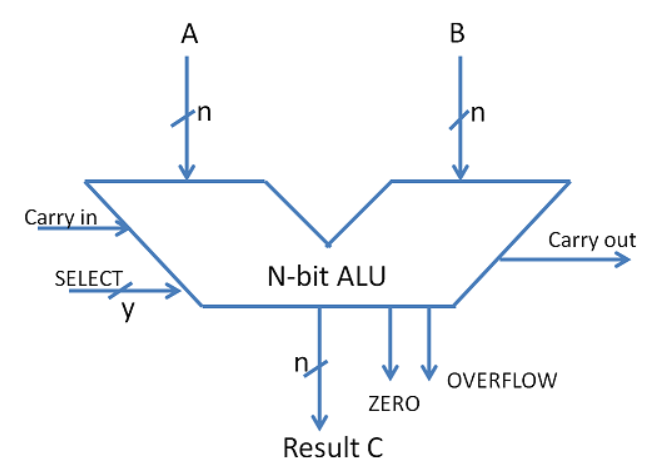
\includegraphics[width=\textwidth]{images/alu.png}
    \caption{ULA}
\end{figure}

Este trabalho tem como objetivo o desenvolvimento de uma ALU de 8 bits utilizando a linguagem de descrição de hardware VHDL, respeitando os princípios de design digital combinacional. O projeto foi implementado no ambiente Quartus II 9.1sp2, sendo exclusivamente composto por código concorrente, sem a utilização de elementos sequenciais como flip-flops ou latches. A ALU implementada é capaz de realizar 16 operações distintas, incluindo operações aritméticas com e sem carry, operações lógicas bit a bit, rotações e deslocamentos.

O relatório está organizado da seguinte forma: na seção 2 são apresentados os requisitos do projeto; a seção 3 descreve o desenvolvimento da ALU, incluindo decisões de projeto e trechos de código relevantes; a seção 4 detalha os testes realizados e os resultados obtidos; por fim, a seção 5 apresenta as considerações finais.